\section{Resultados}
Se obtuvo Neuralyrics, una aplicación web con inteligencia artificial en línea funcional para la generación de nuevas letras musicales pop para ayudar a artistas en necesidad de ideas para generar nuevas canciones y un modelo entrenado con el 2.5\% del dataset original.\\
El algoritmo para llamar al modelo consta de dos elementos esenciales para generar la letra: estructura y semántica.\\
Se evaluó al algoritmo con la precisión que arrojó al modelo que fue un 58\%, esto indica que por cada palabra que se predice, hay una probabilidad muy alta de que sea muy parecida a otra canción existente, dato que nos indica la probabilidad de que con un modelo entrenado con más canciones pueda tener una precisión más baja y pueda generar una palabra verdaderamente al azar y con una semántica correcta. Igualmente se obtuvieron registros de las interacciones de los usuarios en la página web para poder analizar las partes que fueron relevantes y cuánto impacto se tiene en el internet.
\begin{figure}[h]
	\centering
	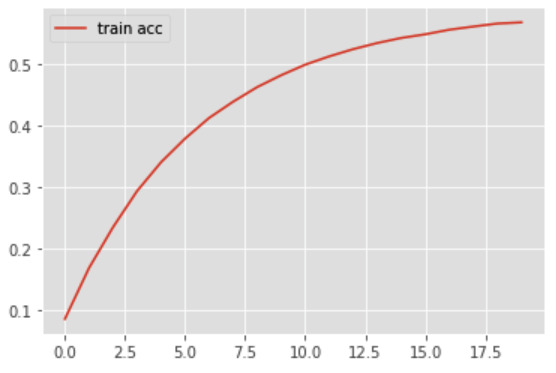
\includegraphics[width=8cm]{figuras/Graficapre.png}
	\caption{Gráfica sobre la presición del modelo}
	\label{fig:Gráfica sobre la presición del modelo}
\end{figure}
\subsection{Demostración online}
Una demostración online para la generación de letras musicales esta disponible en neuralyrics.com esta herramienta fue creada para:
(1) poner el generador a disposición del público, (2) proporcionar
los usuarios formas fáciles de personalizar las letras generadas, y
(3) recopile registros de uso limitado para evaluar y mejorar el algoritmo. El sitio web se lanzó en noviembre del
2021.